\documentclass[border=10pt]{standalone}
\usepackage[svgnames]{xcolor}
\usepackage{amsmath}
\usepackage{pgfplots}
\pgfplotsset{compat=newest}
\usepackage[sfdefault]{FiraSans}
\usepackage{FiraMono}
\renewcommand*\familydefault{\sfdefault}
\begin{document}
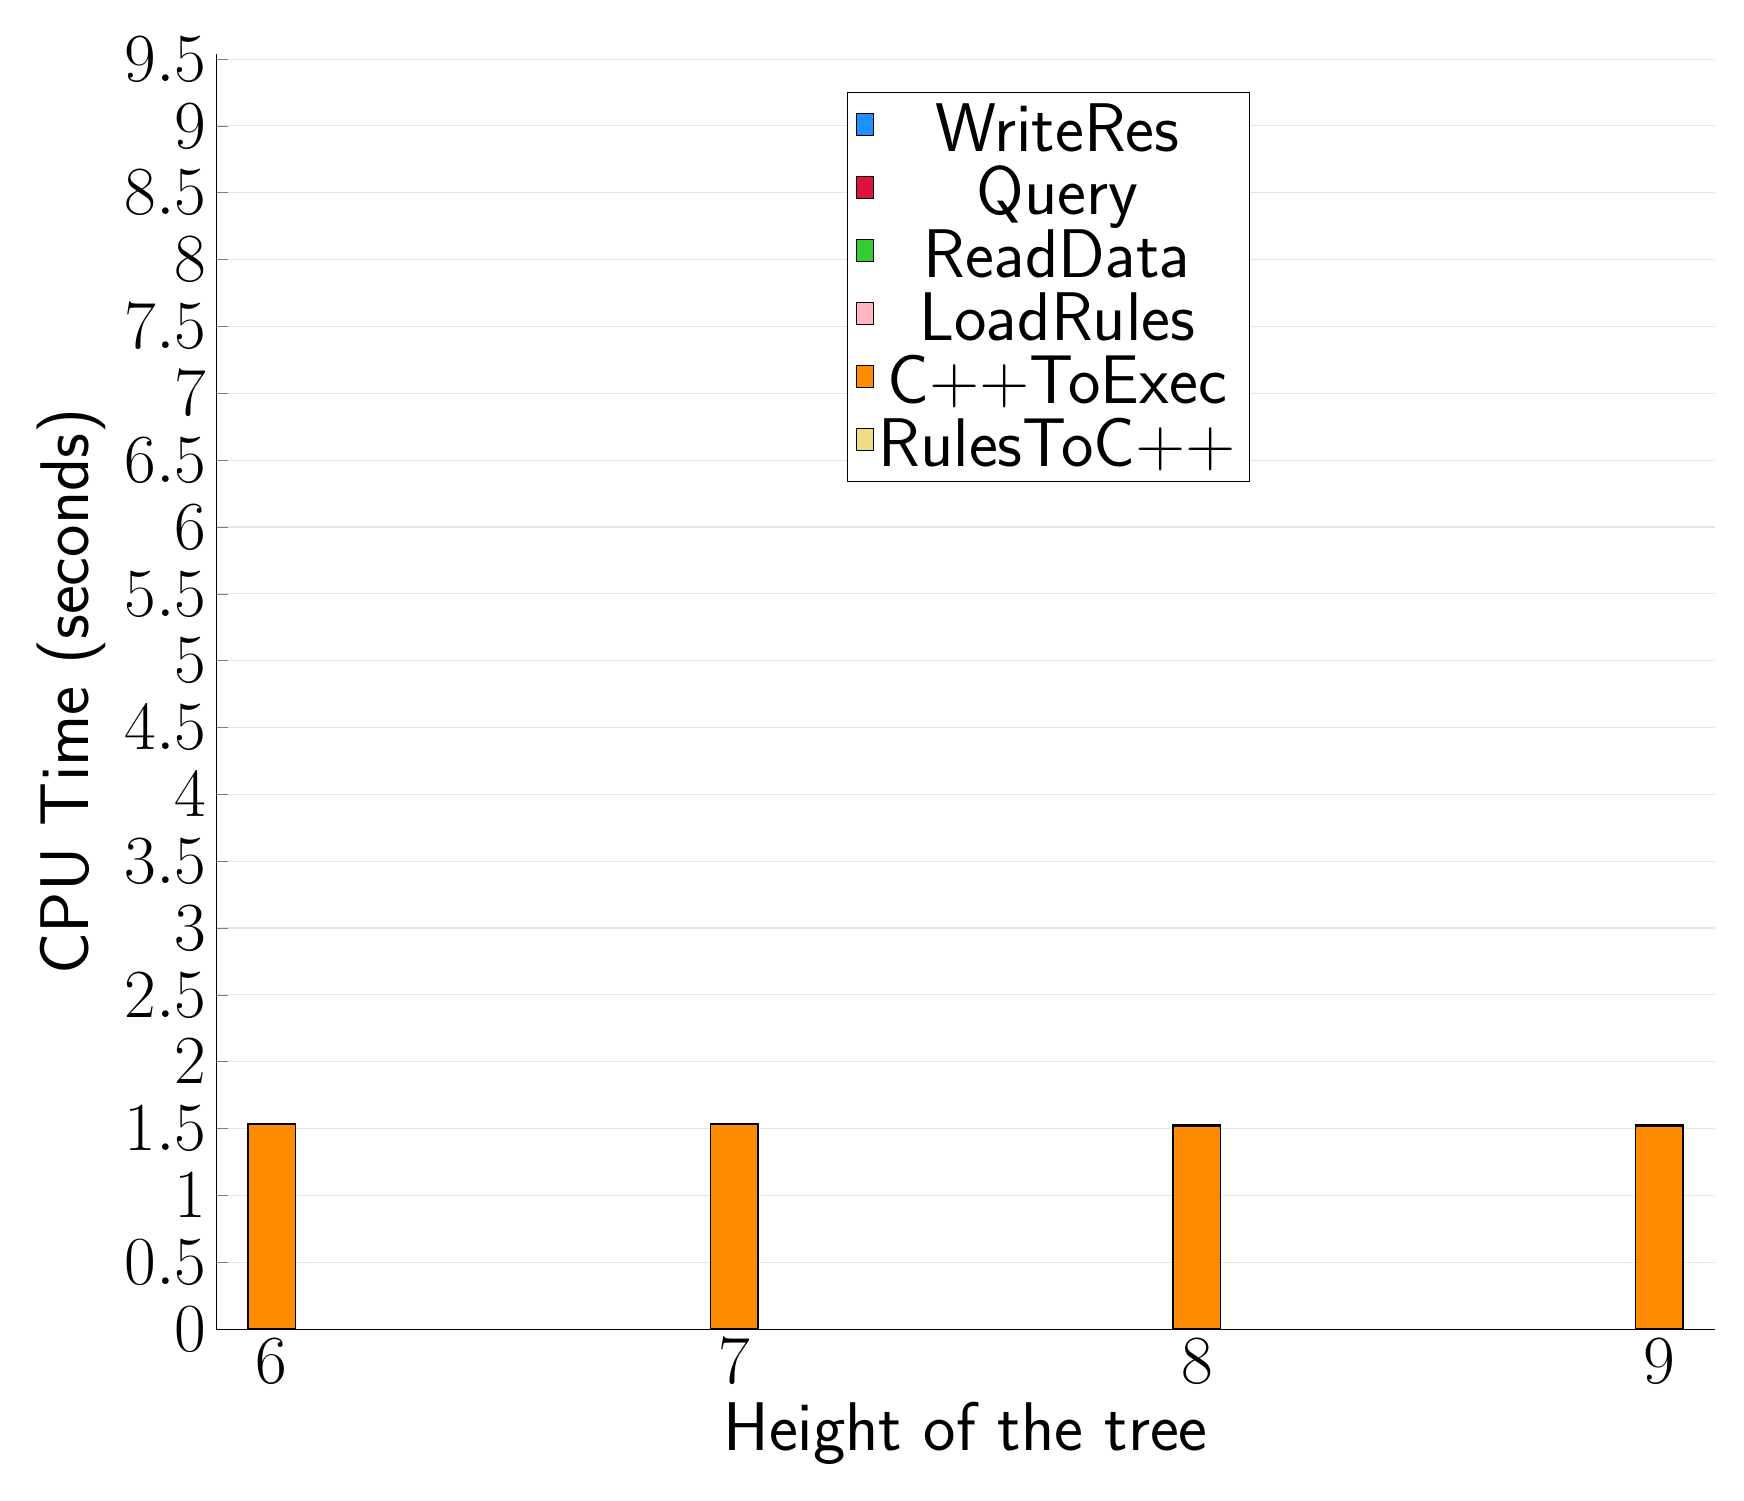
\begin{tikzpicture}
\begin{axis}[
   ybar stacked,
   width=1.7\textwidth,
   bar width=0.6cm,
   ymajorgrids, tick align=inside,
   major grid style={draw=gray!20},
   xtick=data,
   ymin=0, ymax=9.54,
   axis x line*=bottom,
   axis y line*=left,
   enlarge x limits=0.04,
   legend style={
       at={(0.69, 0.97)},
       anchor=north east,
       legend columns=1,
       font=\Huge,
   },
   ylabel={CPU Time (seconds)},
   xlabel={Height of the tree},
   label style={font=\Huge},
   tick label style={font=\Huge},
]
\addlegendimage{fill=DodgerBlue, draw=black, line width=0.2pt}
\addlegendentry{WriteRes}
\addlegendimage{fill=Crimson, draw=black, line width=0.2pt}
\addlegendentry{Query}
\addlegendimage{fill=LimeGreen, draw=black, line width=0.2pt}
\addlegendentry{ReadData}
\addlegendimage{fill=LightPink, draw=black, line width=0.2pt}
\addlegendentry{LoadRules}
\addlegendimage{fill=DarkOrange, draw=black, line width=0.2pt}
\addlegendentry{C++ToExec}
\addlegendimage{fill=LightGoldenrod, draw=black, line width=0.2pt}
\addlegendentry{RulesToC++}
\addplot +[fill=LightGoldenrod, draw=black, line width=0.55pt] coordinates {
(6, 0.0020000000000000005)
(7, 0.0)
(8, 0.0)
(8, 0.0)
(8, 0.0)
(9, 0.0)
(9, 0.0)
(9, 0.0)
(9, 0.0)
(9, 0.0)
};
\addplot +[fill=DarkOrange, draw=black, line width=0.55pt] coordinates {
(6, 1.53)
(7, 1.53)
(8, 1.518)
(8, 1.522)
(8, 1.5180000000000002)
(9, 1.518)
(9, 1.5180000000000002)
(9, 1.516)
(9, 1.514)
(9, 1.516)
};
\addplot +[fill=LightPink, draw=black, line width=0.55pt] coordinates {
(6, 0.00013)
(7, 0.00014300000000000003)
(8, 0.00014359999999999997)
(8, 0.0001354)
(8, 0.0001402)
(9, 0.0001494)
(9, 0.0001428)
(9, 0.0001408)
(9, 0.0001438)
(9, 0.00014419999999999998)
};
\addplot +[fill=LimeGreen, draw=black, line width=0.55pt] coordinates {
(6, 0.0006272000000000001)
(7, 0.0009841999999999997)
(8, 0.0014634)
(8, 0.0014494)
(8, 0.0014785999999999998)
(9, 0.0023426)
(9, 0.0024062)
(9, 0.0023578)
(9, 0.0024032000000000003)
(9, 0.0023315999999999996)
};
\addplot +[fill=Crimson, draw=black, line width=0.55pt] coordinates {
(6, 0.0005461999999999999)
(7, 0.0014252000000000002)
(8, 0.0031812)
(8, 0.0031454000000000005)
(8, 0.0031874)
(9, 0.006167799999999999)
(9, 0.006681000000000001)
(9, 0.006300600000000001)
(9, 0.006572800000000001)
(9, 0.0064984)
};
\addplot +[fill=DodgerBlue, draw=black, line width=0.55pt] coordinates {
(6, 0.0004822)
(7, 0.00048639999999999995)
(8, 0.0005461999999999999)
(8, 0.0004244)
(8, 0.000445)
(9, 0.00046599999999999994)
(9, 0.00047000000000000004)
(9, 0.0003808)
(9, 0.00045000000000000004)
(9, 0.00045779999999999996)
};
\end{axis}
\end{tikzpicture}

\end{document}
